\documentclass[a4paper]{amsproc}
\usepackage{graphicx}              % to include figures
\usepackage[margin=1in]{geometry}  % set the margins to 1in on all sides
\usepackage{concrete}
\usepackage{kpfonts}
\usepackage{amsmath,amsthm,amssymb,amsfonts}               % great math stuff for blackboard bold, etc
\usepackage[svgnames]{xcolor}									% Enabling colors by their 'svgnames'
\usepackage{hyperref}

% various theorems, numbered by section

%%%%%%%%%%%%%%%%%%%%%%%%%%%%%% Textclass specific LaTeX commands.
 \theoremstyle{plain}
 \newtheorem{thm}{Theorem}[section]
 \numberwithin{equation}{section} %% Comment out for sequentially-numbered
 \numberwithin{figure}{section} %% Comment out for sequentially-numbered
 \theoremstyle{plain}
 \newtheorem*{thm*}{Theorem}
 \theoremstyle{definition}
 \newtheorem{example}[thm]{Example}
 \theoremstyle{definition}
 \newtheorem{xca}[section]{Exercise}%%Delete [section] for sequential numbering
 \theoremstyle{remark}
 \newtheorem{rem}[thm]{Remark}

%%% Headers and footers
\usepackage{fancyhdr}												% Needed to define custom headers/footers
	\pagestyle{fancy}												% Enabling the custom headers/footers
\usepackage{lastpage}	
% Footer (you may change this to your own needs)
\lfoot{\footnotesize \texttt{www.albohessab.weebly.com} \textbullet }

%%%%%%%%%%%%%%%%%%%%%%%%%%%%%% User specified LaTeX commands.
\title{\textbf{L'H\^{o}pital's Rule}}

\author{Miliyon T.}
\address{
Department of Mathematics \\ % \hfill (Received 00 00 2010)\\
Addis Ababa University   \\ %\hfill (Revised  00 00 2010)\\
Addis Ababa\\
Ethiopia}
\email{miliyon@ymail.com}

\begin{document}

\maketitle
\nocite{}



\section{Introduction}

Suppose there are continuous functions $f(x)$ and $g(x)$ that are both zero at $x=a$. Then,
the limit $\lim_{x \to a}{\frac{f(x)}{g(x)}}$ cannot be found, since substituting $x=a$ yields $0/0$ which cannot be evaluated.
We use $0/0$ as a notation for an expression known as an \textbf{\textit{indeterminate form}}. A limit is \textit{indeterminate}
if it is one of the following forms
\[
\frac{0}{0},\quad \frac{\pm\infty }{\pm\infty },\quad 1^{\infty },\quad \infty -\infty ,\quad 0\times \infty ,\quad 0^{0},\quad 0^{\infty },\quad \mathrm{or}\quad \infty ^{0.}\]
By some standard algebraic tricks, any of the other forms can be reduced to
one of the first two (though the last two should be kept separate). In some cases, limits that lead to
indeterminate forms may be evaluated by cancellation or rearrangement of terms \cite{Jun}.
However, this does not always work. For example, how would you evaluate $\lim_{x \to 0}{\frac{\sin{x}}{x}}$? Obviously,
inserting $x=0$ will yield an indeterminate form of $0/0$ and in this case, you can neither use algebraic manipulation nor
rearrangement of terms to reduce this expression into a form that yields a valid limit.


\section{Mean Value Theorem}
\begin{thm}[Maximum Minimum, Extreme Value]
Let $f$ be continuous on a closed interval $[a,b]$. Then $f$ has a maximum and a minimum value on $[a,b]$. 
\end{thm}

\begin{proof}

\end{proof}

\begin{thm}[Fermat's Theorem]
Let $f$ be defined on $[a,b]$. If an extreme value of $f$ on $[a,b]$ occurs at a number $c$ in $(a,b)$ at which $f$ has derivative, 
then $f'(c)=0$.
\end{thm}
\begin{proof}
It suffices to show that $f$ does not assume an extreme value at any number $c$ in $(a,b)$ such that $f'(c)$ exists and $f'(c)\neq 0$. 
Therefore we assume that $f'(c)\neq 0$. Consider first the case in which $f'(c)>0$. Since
\[
f'(c)=\lim_{x\to c}\frac{f(x)-f(c)}{x-c}>0
\] 

\end{proof}

\begin{thm}[Rolle's Theorem]\label{thm:rolle}
Let $f$ be continuous on $[a, b]$ and differentiable on $(a, b)$. If $f(a) = f(b)$, then there exists a number
$c \in (a, b)$ such that $f'(c) = 0$.
\end{thm}

\begin{proof}
If $f$ is constant, then its derivative is $0$, so that $f'(c)=0$ for each $c$ in $(a,b)$\footnote{If maximum and minimum both occur at the endpoints, then
$f(x)=f(a)=f(b)$ at every point in $[a,b]$. Hence the function is a horizontal line, and it has derivative zero everywhere on $(a,b)$. We may choose any $c$ at all to get $f'(c)=0$.}.
%\footnote{The proof of theorem \ref{thm:rolle} is based on the fact that if a differentiable function $f$ has a local extrema at a point $x = \zeta$ then $f'(\zeta) = 0$.}
%The idea of the proof is to argue that if $f(a)= f(b)$, then $f$ must attain either a maximum or a minimum somewhere between $a$ and $b$, say at $c$, and the function must
change from increasing to decreasing (or the other way around) at $c$. In particular, if the derivative exists, it must be zero at $c$.
\begin{figure}[htb!]
\centering
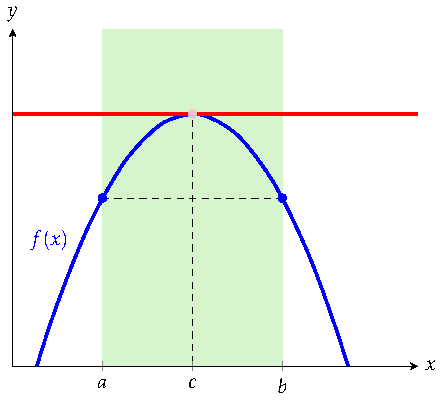
\includegraphics[width=0.3\textwidth]{Rollee}
\caption{Illustration of Rolle's Theorem}
\label{fig:rolle}
\end{figure}

If $f$ is not constant, then its maximum and minimum vales(which exist by Maximum-Minimum(Extreme value) Theorem) are distinct.
Since $f(a)=f(b)$, at least one these values occur at a point $c$ in $(a,b)$. By hypothesis, $f$ is differentiable at $c$, so $f'(c)=0$
by Fermat's Theorem.
%By assumption, $f$ is continuous on $[a,b]$, and by the  extreme value theorem attains both its maximum
%and its minimum in $[a,b]$. If these are both attained at the endpoints of $[a,b]$, then $f$ is  constant on $[a,b]$ and
%so the derivative of $f$ is zero at every point in $(a,b)$.\\ Suppose then that the maximum is obtained at an interior point
%$c$ of $(a,b)$ (the argument for the minimum is very similar, just consider $-f$). We shall examine the above right-
%and left-hand limits separately.\\ For a real $h$ such that $c+h$ is in $[a,b]$, the value $f(c+h)$ is smaller or equal
%to $f(c)$ because $f$ attains its maximum at $c$. Therefore, for every $h>0$,
%\[
%\frac{f(c+h)-f(c)}{h}\le0,
%\]
%hence
%\[
%f'(c+):=\lim_{h \to 0^+}\frac{f(c+h)-f(c)}{h}\le0,
%\]
%where the limit exists by assumption, it may be minus infinity. Similarly, for every $h<0$, the inequality turns around because the denominator is now negative and we get
%\[\frac{f(c+h)-f(c)}{h}\ge0,\]
%hence
%\[
%f'(c-):=\lim_{h \to 0^-}\frac{f(c+h)-f(c)}{h}\ge0,
%\]
%where the limit might be plus infinity.\\ Finally, when the above right and left-hand limits agree (in particular when $f$ is differentiable), then the derivative of $f$ at $c$ must be zero.
\end{proof}

\section{Extended Mean Value Theorem}


%\begin{rem}\color{red}
%If $f$ is a function as above but $f(a) = f(b) = c$ then the conclusion of Rolle's theorem still applies. In other words, theorem
%\ref{thm:rolle} applies whenever $f(a) = f(b)$.
%\end{rem}

\begin{thm}[Cauchy]
Let $f$ and $g$ be differentiable on $(a, b)$ and continuous on $[a, b]$. Suppose that $g(x)=0$   in $(a, b)$. Then there is at least one point $c$ in $(a, b)$ such that
\[\frac{f'(c)}{g'(c)}=\frac{f(b)-f(a)}{g(b)-g(a)}\]
\end{thm}

\begin{proof}
The proof of Cauchy's mean value theorem is based on the same idea as the proof of the mean value theorem.
First we need to define a new function that satisfies the conditions of Rolle's theorem. Define the function $h$ by
\[
h(x)=\bigl(f(b)-f(a)\bigr)\bigl(g(x)-g(a)\bigr)-\bigl(g(b)-g(a)\bigr)\bigl(f(x)-f(a)\bigr),
\]
which is continuous on $[a,b]$ and differentiable on $(a,b)$. Then
\[
h(a)=\bigl(f(b)-f(a)\bigr)\bigl(g(a)-g(a)\bigr)-\bigl(g(b)-g(a)\bigr)\bigl(f(a)-f(a)\bigr)=0
\]
and
\[
h(b)=\bigl(f(b)-f(a)\bigr)\bigl(g(b)-g(a)\bigr)-\bigl(g(b)-g(a)\bigr)\bigl(f(b)-f(a)\bigr)=0,
\]
so $h(a)=h(b)$ and Rolle's theorem applies. The derivative of $h$ is
\[
h'(x)=\bigl(f(b)-f(a)\bigr)g'(x) - \bigl(g(b)-g(a)\bigr)f'(x)
\]
and Rolle's theorem states that it is equal to zero at some point, i.e., $h'(c)=0$ for some $c\in (a,b)$. The equation for the derivative at $c$ is
\[
h'(c)=\bigl(f(b)-f(a)\bigr)g'(c) - \bigl(g(b)-g(a)\bigr)f'(c)=0,
\]
therefore
\[
\bigl(f(b)-f(a)\bigr)g'(c) = \bigl(g(b)-g(a)\bigr)f'(c).
\]
If $g'(c)$ and $g(b)-g(a)$ are non-zero this can be written as
\[\frac{f'(c)}{g'(c)} = \frac{f(b)-f(a)}{g(b)-g(a)}.\]
\end{proof}

\section{L'H\^{o}pital's Rule}\footnote{In the 17th and 18th centuries, the name was commonly spelled "l'Hospital",
and he himself spelled his name that way. However, French spellings have been altered: the silent 's' has been removed and replaced
with the circumflex over the preceding vowel. The former spelling is still used in English where there is no circumflex}

\begin{thm}[L'H\^{o}pital's Rule, \(0/0\) form]
Let \( f \) and \( g \) be differentiable on some interval, with \( a \) in that interval, and assume they satisfy
\[\lim _{x\rightarrow a}f(x)=0,\, \, \mathrm{and}\, \, \lim _{x\rightarrow a}g(x)=0.\]
 Then,
\[\lim _{x\rightarrow a}\frac{f(x)}{g(x)}=\lim _{x\rightarrow a}\frac{f'(x)}{g'(x)}.\]
\end{thm}
\begin{proof}
This result uses the Generalized MVT from the previous section. Let's deal with limits on the right. Assume that
\[
\lim _{x\rightarrow a+}f(x)=0,\, \, \mathrm{and}\, \, \lim _{x\rightarrow a+}g(x)=0,
\]
and that \( f \) and \( g \) are differentiable on some interval \( (a,b). \) If you set \( g(a)=f(a)=0 \), then the functions \( f \)
and \( g \) will be continuous on \( [a,b] \) and differentiable on \( (a,b) \), so will fit the hypotheses of the generalized MVT.
Now, there should be some question about the hypothesis that \( g'(x)\neq 0 \), but certainly the limit
\[
\lim _{x\rightarrow a+}\frac{f'(x)}{g'(x)}
\]
won't make sense unless \( g'(x)\neq 0 \) on some interval near \( a \), so we can choose \( b \) so that \( g'(x)\neq 0 \) on
\( (a,b) \). Then, by the generalized MVT, if \( x\in (a,b) \),
\begin{eqnarray*}
\frac{f(x)}{g(x)} & = &\frac{f(x)-f(a)}{g(x)-g(a)}\\
                  & = &\frac{\tfrac{f(x)-f(a)}{x-a}}{\tfrac{g(x)-g(a)}{x-a}}\\
                  & = &\frac{f'(c)}{g'(c)},
\end{eqnarray*}
for some \( c \) between \( a \) and \( x \). Since \( c \) is trapped between \( a \) and \( x \), as \( x \) approaches \( a \),
\( c \) will also approach \( a \), and so
\begin{eqnarray*}
\lim _{x\rightarrow a+}\frac{f(x)}{g(x)} & = & \lim _{c\rightarrow a+}\frac{f'(c)}{g'(c)}\\
 & = & \lim _{x\rightarrow a+}\frac{f'(x)}{g'(x)}.
\end{eqnarray*}
Since the same ideas work out for the limits from the left, the statement follows.
\end{proof}

\begin{thm}[L'H\^{o}pital's Rule, $\infty /\infty$ form]
Let \( f \) and \( g \) be differentiable on some interval, with \( a \) in that interval, and assume they satisfy
\[\lim _{x\rightarrow a}f(x)=\infty ,\, \, \mathrm{and}\, \, \lim _{x\rightarrow a}g(x)=\infty .\]
Then,
\[\lim _{x\rightarrow a}\frac{f(x)}{g(x)}=\lim _{x\rightarrow a}\frac{f'(x)}{g'(x)}.\]
\end{thm}
\begin{proof}
Due to the fact that the ± sign is nothing more than a multiplicative factor valued at $\pm1$ , it is a constant and a scalar which
may be factored out of the limits. Consequently, the rule which applies to the indeterminate form $\tfrac{\infty}{\infty}$ also applies
to $\tfrac{-\infty}{\infty}\ ,\ \tfrac{\infty}{-\infty}\ ,\ \tfrac{-\infty}{-\infty}$. We may assume now that as $x\to a$ , our
functions $f(x),g(x)$ both, separately, approach an infinite magnitude.
\[\lim_{x\to a}\frac{f(x)}{g(x)}\to\frac{\infty}{\infty}\]
What we may do is perform algebraic manipulations. We shall copy from the following algebraic rule
\[\frac{a}{b}=\frac{\frac1b}{\frac1a}\]
As it pertains to the limit in question
\[\lim_{x\to a}\frac{\frac1{g(x)}}{\frac1{f(x)}}\]
Now, even though the functions $f,g$ approach infinite magnitudes, their reciprocals approach zero from the positive.
\[\lim_{x\to a}\frac{\frac{1}{g(x)}}{\frac{1}{f(x)}}\to\frac{\frac{1}{\infty}}{\frac{1}{\infty}}=\frac{0^+}{0^+}\]
We are now in an indeterminate form $\tfrac00$ , and L'H\^{o}pital's Rule for $\tfrac00$ applies.
\[\lim_{x\to a}\frac{\frac{d}{dx}\frac1{g(x)}}{\frac{d}{dx}\frac{1}{f(x)}}\]
Evaluate the derivatives, applying the chain rule.
\[\lim_{x\to a}\frac{-\frac{g'(x)}{g(x)^2}}{-\frac{f'(x)}{f(x)^2}}\]
Simplify
\[\lim_{x\to a}\frac{f(x)^2\cdot g'(x)}{g(x)^2\cdot f'(x)}\]
We have thus far proved the last equality. We may apply the various limit properties in order to rearrange the functions. We can end
up with
\[\lim_{x\to a}\frac{f(x)}{g(x)}=\lim_{x\to a}\frac{f'(x)}{g'(x)}\]
\end{proof}
\begin{table}[ht]
\centering
\resizebox{\textwidth}{!}{
\begin{tabular}{|c|l|l|l|}
\hline
Indeterminate form & Conditions & Transformation to $0/0$ & Transformation to $\infty/\infty$  \\ \hline
$0/0$              & \(\displaystyle\lim_ {x \to c} f(x)=0,\ \displaystyle\lim_ {x \to c} g(x)=0\) & \_ & $ \displaystyle\lim_ {x \to c} \frac{f(x)}{g(x)}=\displaystyle\lim_ {x \to c} \frac{1/g(x)}{1/f(x)}$  \\ \hline
  $\infty/\infty$    & $ \displaystyle\lim_ {x \to c} f(x)=\infty,\  \displaystyle\lim_ {x \to c} g(x)=\infty$ & $ \displaystyle\lim_ {x \to c} \frac{f(x)}{g(x)} = \displaystyle\lim_ {x \to c} \frac{1/g(x)}{1/f(x)}$   & \_ \\ \hline
  $0\cdot\infty$     & $ \displaystyle\lim_ {x \to c} f(x) = 0,\  \displaystyle\lim_ {x \to c} g(x) = \infty $ & $ \displaystyle\lim_ {x \to c} f(x)g(x) = \displaystyle\lim_ {x \to c} \frac{f(x)}{1/g(x)}$ & $ \displaystyle\lim_ {x \to c} f(x)g(x) = \displaystyle\lim_ {x \to c} \frac{g(x)}{1/f(x)}   $  \\ \hline
  $\infty-\infty$    & $ \displaystyle\lim_ {x \to c} f(x) = \infty,\  \displaystyle\lim_ {x \to c} g(x) = \infty   $ & $ \displaystyle\lim_ {x \to c} (f(x) - g(x)) = \displaystyle\lim_ {x \to c} \frac{1/g(x) - 1/f(x)}{1/(f(x)g(x))}   $ & $ \displaystyle\lim_ {x \to c} (f(x) - g(x)) = \ln \displaystyle\lim_ {x \to c} \frac{e^{f(x)}}{e^{g(x)}}   $ \\ \hline
  $0^0$              & $ \displaystyle\lim_ {x \to c} f(x) = 0^+, \displaystyle\lim_ {x \to c} g(x) = 0   $ & $ \displaystyle\lim_ {x \to c} f(x)^{g(x)} = \exp \displaystyle\lim_ {x \to c} \frac{g(x)}{1/\ln f(x)}   $ &$ \displaystyle\lim_ {x \to c} f(x)^{g(x)} = \exp \displaystyle\lim_ {x \to c} \frac{\ln f(x)}{1/g(x)}   $  \\ \hline
  $1^{\infty}$       & $ \displaystyle\lim_ {x \to c} f(x) = 1,\  \displaystyle\lim_ {x \to c} g(x) = \infty   $ & $ \displaystyle\lim_ {x \to c} f(x)^{g(x)} = \exp \displaystyle\lim_ {x \to c} \frac{\ln f(x)}{1/g(x)}   $ & $ \displaystyle\lim_ {x \to c} f(x)^{g(x)} = \exp \displaystyle\lim_ {x \to c} \frac{g(x)}{1/\ln f(x)}   $ \\ \hline
  $0^{\infty}$     & $ \displaystyle\lim_ {x \to c} f(x) = \infty,\  \displaystyle\lim_ {x \to c} g(x) = 0   $ & $ \displaystyle\lim_ {x \to c} f(x)^{g(x)} = \exp \displaystyle\lim_ {x \to c} \frac{g(x)}{1/\ln f(x)}   $ & $ \displaystyle\lim_ {x \to c} f(x)^{g(x)} = \exp \displaystyle\lim_ {x \to c} \frac{\ln f(x)}{1/g(x)}   $  \\
  \hline
\end{tabular}}
\caption{Indeterminate forms and their transformations for applying L'H\^{o}pital's rule}\label{tabel:1}
\end{table}
\section{Worked Examples}

\begin{example}[$0/0$]\label{exm:1}
Evaluate the limit \[\lim_{x\to 0}\frac{\sin x}{x} \].
\end{example}

\begin{proof}[Solution]
Let \( f(x)=\sin x \) and \( g(x)=x \). Then we have \( \lim_{x\to 0}f(x)=\lim_{x\to 0}g(x)=0 \), \( f^{\prime}(x)=\cos x \), and \( g^{\prime}(x)=1 \). Since \[ \lim_{x\to 0}\frac{f^{\prime}(x)}{g^{\prime}(x)}=\lim_{x\to 0}\frac{\cos x}{1}=1, \] according to L'H\^{o}pital's theorem we have \[ \lim_{x\to 0}\frac{f(x)}{g(x)}=\lim_{x\to 0}\frac{\sin x}{x}=1.\]
\end{proof}

\begin{rem}[\textbf{Circular Reasoning}]\color{red}
By the definition of the derivative,
\[\frac{d}{dx}\sin x = \lim_{h\to0}\frac{\sin(x+h)-\sin(x)}{h}\]
Using the fact that $\sin A- \sin B = 2\cos(\frac{A+B}{2})\sin(\frac{A-B}{2}),$
\begin{align*}
\frac{d}{dx} \sin x &= \lim_{h\to0}2\cos(x+\frac{h}{2}) \frac{\sin\frac{h}{2}}{h}\\
                    &= \lim_{h\to0} \cos(x+\frac{h}{2}) \frac{\sin\frac{h}{2}}{\frac{h}{2}}\\
                    &=\cos x\lim_{h\to0}\frac{\sin\frac{h}{2}}{\frac{h}{2}}
\end{align*}
We are now forced to evaluate an expression of the form $\frac{\sin x}{x}$ as x tends to 0. By the Squeeze Theorem, we know this limit is $1$, proving that the derivative of $\sin x$ is indeed $\cos x$. Thus, using L'H\^{o}pital's theorem to prove that \( \sin x/x\to 1 \) would create a logical error called circular reasoning. Namely, the evaluation of the limit \( \lim_{x\to0}\frac{\sin x}x \) requires us to know that the derivative of \( \sin x \) is equal to \( \cos x \). This result was proved using the fact that \( \lim_{x\to 0}\frac{\sin x}x=1 \).\\ However, if we know that \( (\sin x)^{\prime}=\cos x \), then Example \ref{exm:1} is a correct application of L'H\^{o}pital's theorem to prove that \(  \lim_{x\to 0}\frac{\sin x}x=1 \). The trouble is that all those who know that \( (\sin x)^{\prime}=\cos x \) probably already know that \( \frac{\sin x}x\to 1 \) as \( x\to 0 \).
\end{rem}

\begin{example}[$0^0$]\label{exm:2}
Evaluate the limit \(  \lim_{x\to 0^+}x^x \).
\end{example}

\begin{proof}[Solution]
Let us first rewrite \(  x^x=e^{\ln(x^x)}=e^{x\ln x} \). Since \( f(z)=e^z \) is a continuous function, it suffices to find the limit \(  \lim_{x\to 0^+}x\ln x \).
\begin{eqnarray*}
\lim_{x\to 0^+}x\ln x&=&\lim_{x\to 0^+}\frac{\ln x}{\frac1x}.
\end{eqnarray*}
The last limit can be found using L'H\^{o}pital's rule applied to \( g(x)=-\ln x \) and \( h(x)=\frac1x \). Both functions converge to \( +\infty \) and their derivatives satisfy \( g^{\prime}(x)=-\frac1x \) and \( h(x)=-\frac1{x^2} \) hence \(  \lim_{x\to 0^+}\frac{g^{\prime}(x)}{h^{\prime}(x)}=0 \). Thus \(  \lim_{x\to 0^+}x^x=\lim_{x\to 0^+}e^0=1 \).
\end{proof}

\begin{example}[$\infty/\infty$]\label{exm:3}
Evaluate the limit
\[ \lim_{x\to \infty}\frac{e^x}{x^n},\quad n\in\Bbb{N}.\]
\end{example}

\begin{proof}[Solution]
It's in the form of $\infty/ \infty$ so let's apply L'H\^{o}pital's Rule
\[ \lim_{x\to \infty}\frac{e^x}{x^n}=\]

Sometimes we will need to apply L'H\^{o}pital's Rule more than once.
\end{proof}

\begin{example}[$0\cdot -\infty$]\label{exm:4}
Evaluate the following limit.
\[\lim_{x\to 0^+}x\ln x\]
\end{example}

\begin{proof}[Solution]
So, in the limit, we get the indeterminate form $0\cdot -\infty$. L'H\^{o}pital's Rule won't work on products, it only works on
quotients. However, we can turn this into a faction using Table \ref{tabel:1}.
\[\lim_{x\to 0^+}x\ln x=\lim_{x\to 0^+}\frac{\ln x}{1/x}\]
The limit is now in the form $-\infty/\infty$ and we can now use L'H\^{o}pital's Rule. We have
\[
\lim_{x\to 0^+}{  x\ln(x) } = \lim_{x\to 0^+} \frac{\ln(x)}{\frac{1}{x}} = \lim_{x\to 0^+} \frac{x^{-1}}{-x^{-2}} = 0.
\]
\end{proof}

\begin{example}[$\infty\cdot 0$]\label{exm:5}
Evaluate the following limit.
\[\lim_{x\to \infty}xe^x\]
\end{example}

\begin{proof}[Solution]

\end{proof}

\begin{example}[$\infty^0$]\label{exm:6}
Evaluate the following limit.
\[\lim_{x\to \infty}x^{\frac{1}{x}}\]
\end{example}

\begin{proof}[Solution]
In the limit this is the indeterminate form $\infty^0$. The simplest way is to use Table \ref{tabel:1} but let us do this from the scratch.
Let's first define the following.
\[y=x^{\frac{1}{x}}\]
Now, if we take the natural $\log$ of both sides we get,
\[\ln y=\frac{\ln x}{x}\]
Let's now take a look at the following limit.
\[\lim_{x\to \infty}\ln y=\lim_{x\to \infty}\frac{\ln x}{x}=\lim_{x\to \infty}\frac{1/x}{1}=0\]
This limit was just a L'H\^{o}pital's Rule. So, what did this have to do with our limit?
Well first notice that,
\[y=e^{\ln y},\]
and so our limit could be written as,
\[\lim_{x\to \infty}x^{\frac{1}{x}}=\lim_{x\to \infty}y=\lim_{x\to \infty}e^{\ln y}.\]
We can now use the limit above to finish this problem.
\[\lim_{x\to \infty}x^{\frac{1}{x}}=\lim_{x\to \infty}y=\lim_{x\to \infty}e^{\lim_{x\to \infty}\ln y}=e^{0}=1\]
\end{proof}

\begin{example}[$1^\infty$]\label{exm:7}
Find
\[
\lim_{x\to\infty}\left(1+\frac{1}{x}\right)^x
\]
\end{example}

\begin{proof}[Solution]
Plugging the value of $x$ into the limit yields
\[\lim_{x\to\infty}\left(1+\frac{1}{x}\right)^x=1^\infty\]
Let
\[k=\lim_{x\to\infty}\left(1+\frac{1}{x}\right)^x=1^\infty\]
Then
\begin{align*}
\ln(k)&=\lim_{x\to\infty}\ln\left(1+\frac{1}{x}\right)^x\\
      &=\lim_{x\to\infty}x\ln\left(1+\frac{1}{x}\right)\\
      &=\lim_{x\to\infty}\frac{\ln\left(1+\frac{1}{x}\right)}{\frac{1}{x}}=\frac{\ln(1)}{\frac{1}{x}}=\frac{0}{0}
\end{align*}
We now apply L'H\^{o}pital's rule by taking the derivative of the top and bottom with respect to $x$.
\[\frac{d}{dx}\left[\ln\left(1+\frac{1}{x}\right)\right]=\frac{x}{x+1}\cdot\frac{-1}{x^2}=-\frac{1}{x(x+1)}\]
\[\frac{d}{dx}\left(\frac{1}{x}\right)=-\frac{1}{x^2}\]
Returning to the expression above
\begin{align*}
\ln(k) &=\lim_{x\to\infty}\frac{-(-x^2)}{x(x+1)}\\
       &=\lim_{x\to\infty}\frac{x}{x+1}=\frac{\infty}{\infty}
\end{align*}
We apply L'H\^{o}pital's rule once again
\[\ln(k)=\lim_{x\to\infty}\frac{1}{1}=1\]
Therefore
\[k= \lim_{x\to\infty}\left(1+\frac{1}{x}\right)^x=e \]
\end{proof}

\begin{rem}\color{red}
This does not prove that $1^\infty=e$ because
\[\lim_{x\to\infty}\left(1+\frac{2}{x}\right)^x=1^\infty\ne e\]
\end{rem}

\begin{thebibliography}{9}
\bibitem{Jun}
[Larson, Ron and Edwards, Bruce H] Calculus of a single variable, 2013.

\bibitem{amsshort}
[Walter Rudin] Principles of Mathematical Analysis.

\end{thebibliography}
\end{document}
